%!TEX root = spire-project.tex
\subsection{Dust Emission}

To measure the size and mass of optically thick molecular clouds, we can not simply look at the starlight passing through them, we must instead look at the emission from the dust \citep{hildebrand1983determination}. For very cool clouds (\textless 20K) the emission from the dust grains is in the far-infrared and submillimetre wavelengths.

Observations at these wavelengths are generally not possible from ground based telescopes due to atmospheric absorption \citep{houghton2002physics} so instead they are observed from space based observing platforms such as IRAS, Spitzer and Herschel.

\subsection{Blackbody Radiation}

All bodies at finite temperature emit EM radiation; a body in thermal equilibrium with its environment will emit according to a blackbody spectrum. While classical descriptions explained a portion of this radiation, it was not until the early 1900's that Max Planck described this emission fully \citep{planck1914theory}. Planck developed his model using quantum theory, first developing his theory as an improvement to the Wein approximation \citep{wien1897} using empirically measured constants, and later developing a physical derivation by considering the energies of photons inside a box at thermal equilibrium. Planck derived an expression for the spectral radiance of a body, which can be expressed in terms of different spectral variables, e.g. in terms of frequency in equation \ref{bbf} and wavelength, as in equation \ref{bbw}.

\begin{figure}[H]
    \centering
    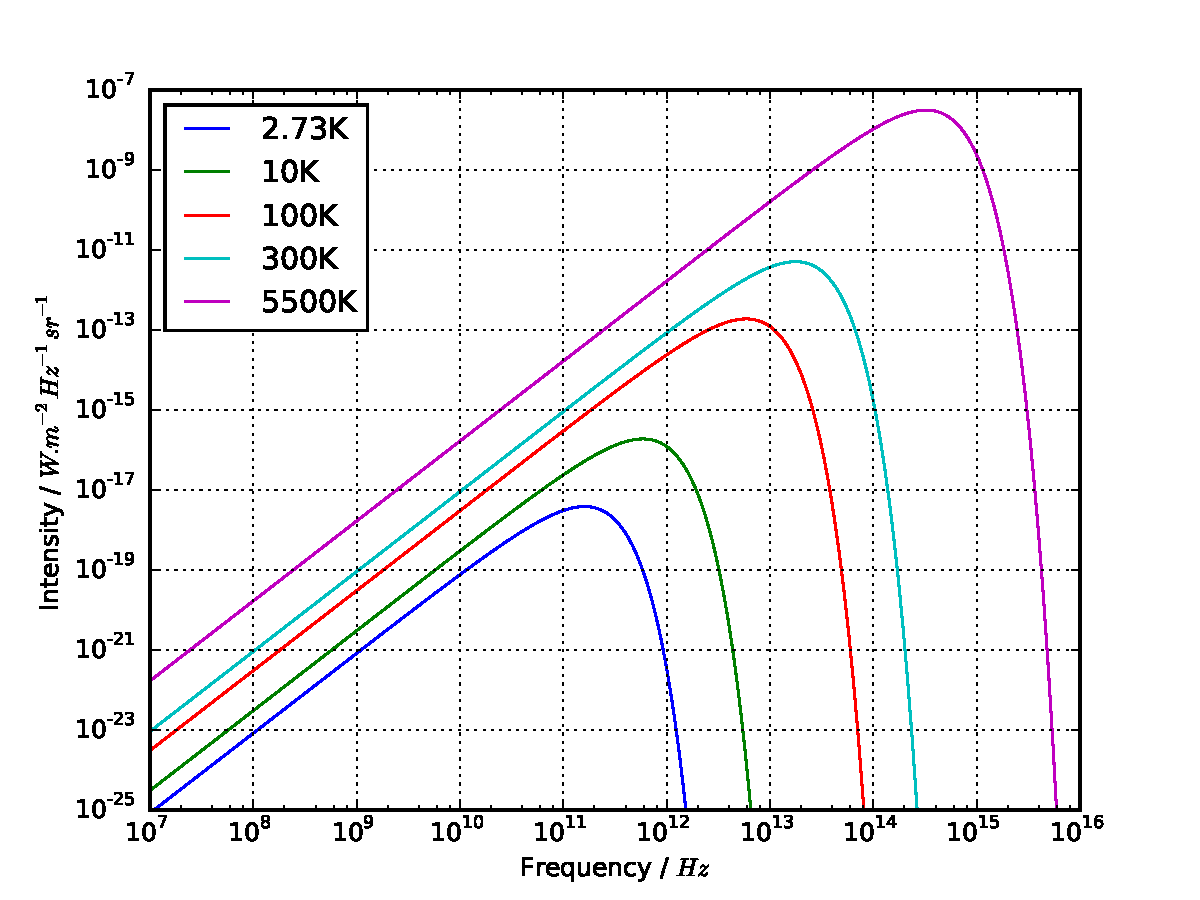
\includegraphics[width=\linewidth]{figures/bb10k.pdf}
    \caption{Blackbody spectrum for bodies at various temperatures}
    \label{bb10k}
\end{figure}

\begin{equation}
    \label{bbf}
    B_\nu(\nu,T) = \frac{2h\nu^3}{c^2}\left( e^{\frac{h\nu}{k_bT}} - 1\right)^{-1}
\end{equation}

\begin{equation}
    \label{bbw}
    B_\lambda(\lambda,T) = \frac{2hc^2}{\lambda^5}\left( e^{\frac{hc}{\lambda k_bT}} - 1\right)^{-1}
\end{equation}

For a blackbody at $10\units{K}$, i.e. typical cold cosmic dust, the spectral radiance will look as shown in Figure \ref{bb10k}, with a peak at approximately $290\units{\mu m}$.

\subsection{How to observe}

\subsubsection{Angular Resolution}

The resolution of any optical system is limited by two factors, aberration and diffraction. Aberrations can be considered to be caused by any defect in the optical system, so can be overcome simply by the use of better construction techniques and use of higher quality materials. In well constructed optical devices, such as modern telescopes, the resolution of any image produced is then limited only by the diffraction of the optical system.

Due to the wave like nature of light, any light passing through an aperture will undergo diffraction. Light from a point source such as a star, passing through a circular aperture will appear in the focal plane as a circular image with a series of rings surrounding it as shown in Figure \ref{airy}. Lord Rayleigh defined a criterion for defining when two objects are resolvable from each other as when the diffraction maximum of one of the objects coincides with the first minimum of the second object \citep{rayleigh1880v}.

\begin{figure}[H]
    \centering
    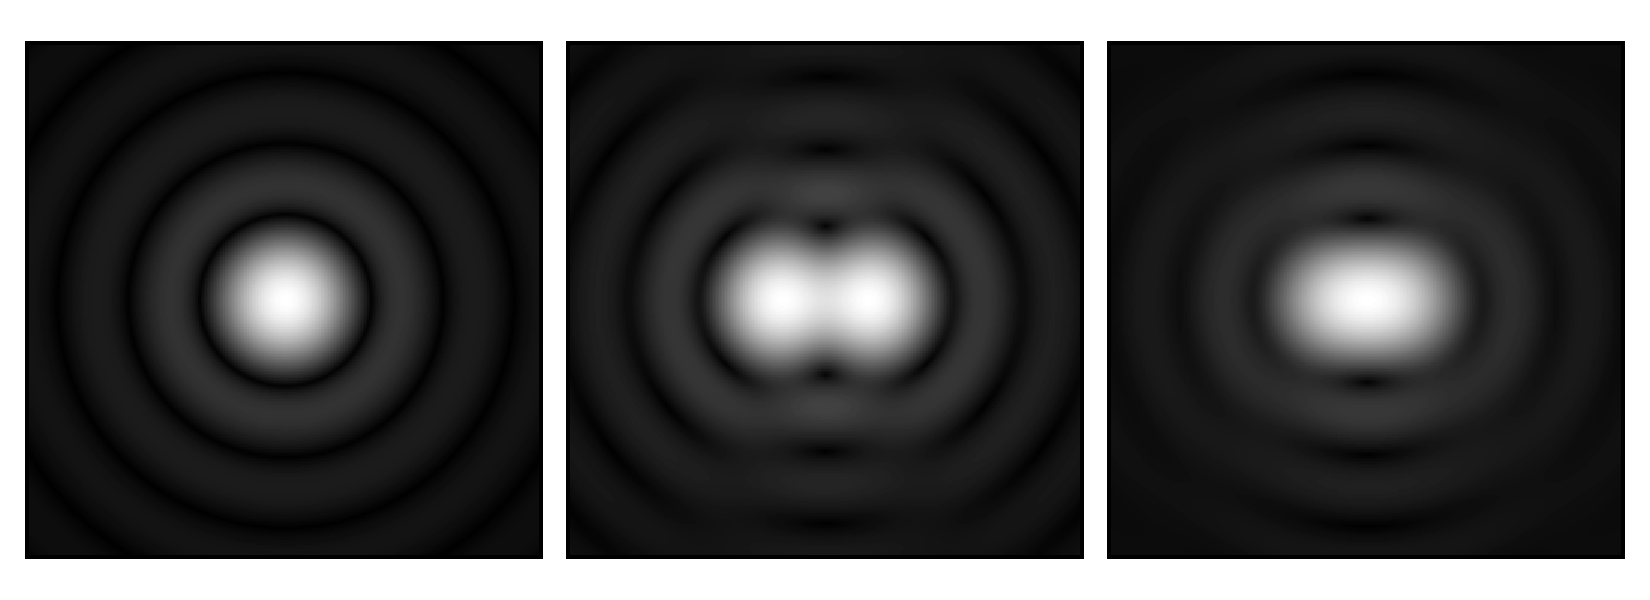
\includegraphics[width=\linewidth]{figures/airy.pdf}
    \caption[Point spread functions]{Point spread functions, from left to right, the Airy disk for a point source, two point sources at the Rayleigh criterion, and two indistinguishable point sources}
    \label{airy}
\end{figure}

Equation \ref{angularres} gives the angular resolution on the sky, as determined by the aperture diameter of the telescope and the wavelength of light. The quality of the images then will increase as $\theta$ decreases, i.e. the angular size of resolvable objects becomes smaller. Clearly as equation \ref{angularres} shows, the resolution then worsens as the wavelength increases, and increases as the diameter of the telescope aperture increases. The telescope beam itself will have a FWHM of approximately $\lambda/D$. As the observation wavelengths are largely determined by the type of objects being observed, the only practical way to improve the the angular resolution is then to increase the telescope aperture size. This of course has the downside of being very expensive, and in the case of space telescopes impractical due to limitations of the launch systems. NASA has a report claiming that the cost of a space telescope is related to the diameter by equation \ref{nasacost} \citep{stahl2011update}.

\begin{equation}
    \theta = 1.22 \frac{\lambda}D
    \label{angularres}
\end{equation}

\begin{equation}
    \text{Cost} \propto D^{1.4}
    \label{nasacost}
\end{equation}

It is therefore very advantageous to find any mechanism to help increase the angular resolution of the observations without incurring additional costs in the telescope construction, or cost of the missions required to launch space telescopes.

\subsubsection{IR detection using Bolometers}

Detection of submillimetre radiation is not possible with CCD technology as is used for imaging in optical and some near optical infra-red detectors \citep{janesick2001scientific}. CCDs work in principle by having electrons released by photo-excitation, and collected into a potential well before measurement. While CCDs have excellent quantum efficiencies (the ratio of incident photons converted to electron-hole pairs) in and around optical wavelength bands, their response falls off around $1\units{\mu m}$ because the photons are no longer energetic enough to produce electron-hole pairs.

Equation \ref{photonenergy} shows that the energy of a photon is inversely proportional to the wavelength. Clearly optical and near infra red photons will have a higher energy than sub millimeter photons, so much so that there is no material that can act as a CCD for submillimetre photons; instead a different method of detection is required.

\begin{equation}
    E = \frac{hc}{\lambda}
    \label{photonenergy}
\end{equation}

Instead of using CCD type devices, one can use bolometers to detect the photons. The principal mechanism of bolometer operation is different to CCDs in that it does not rely on the excitation of electrons (Figure \ref{bolometer}). Instead, as the photons do not have high enough energy, they simply cause atoms in some absorbing material to become thermally excited. This action then changes the resistivity of the material which is something that can be measured.

\begin{figure}[H]
    \centering
    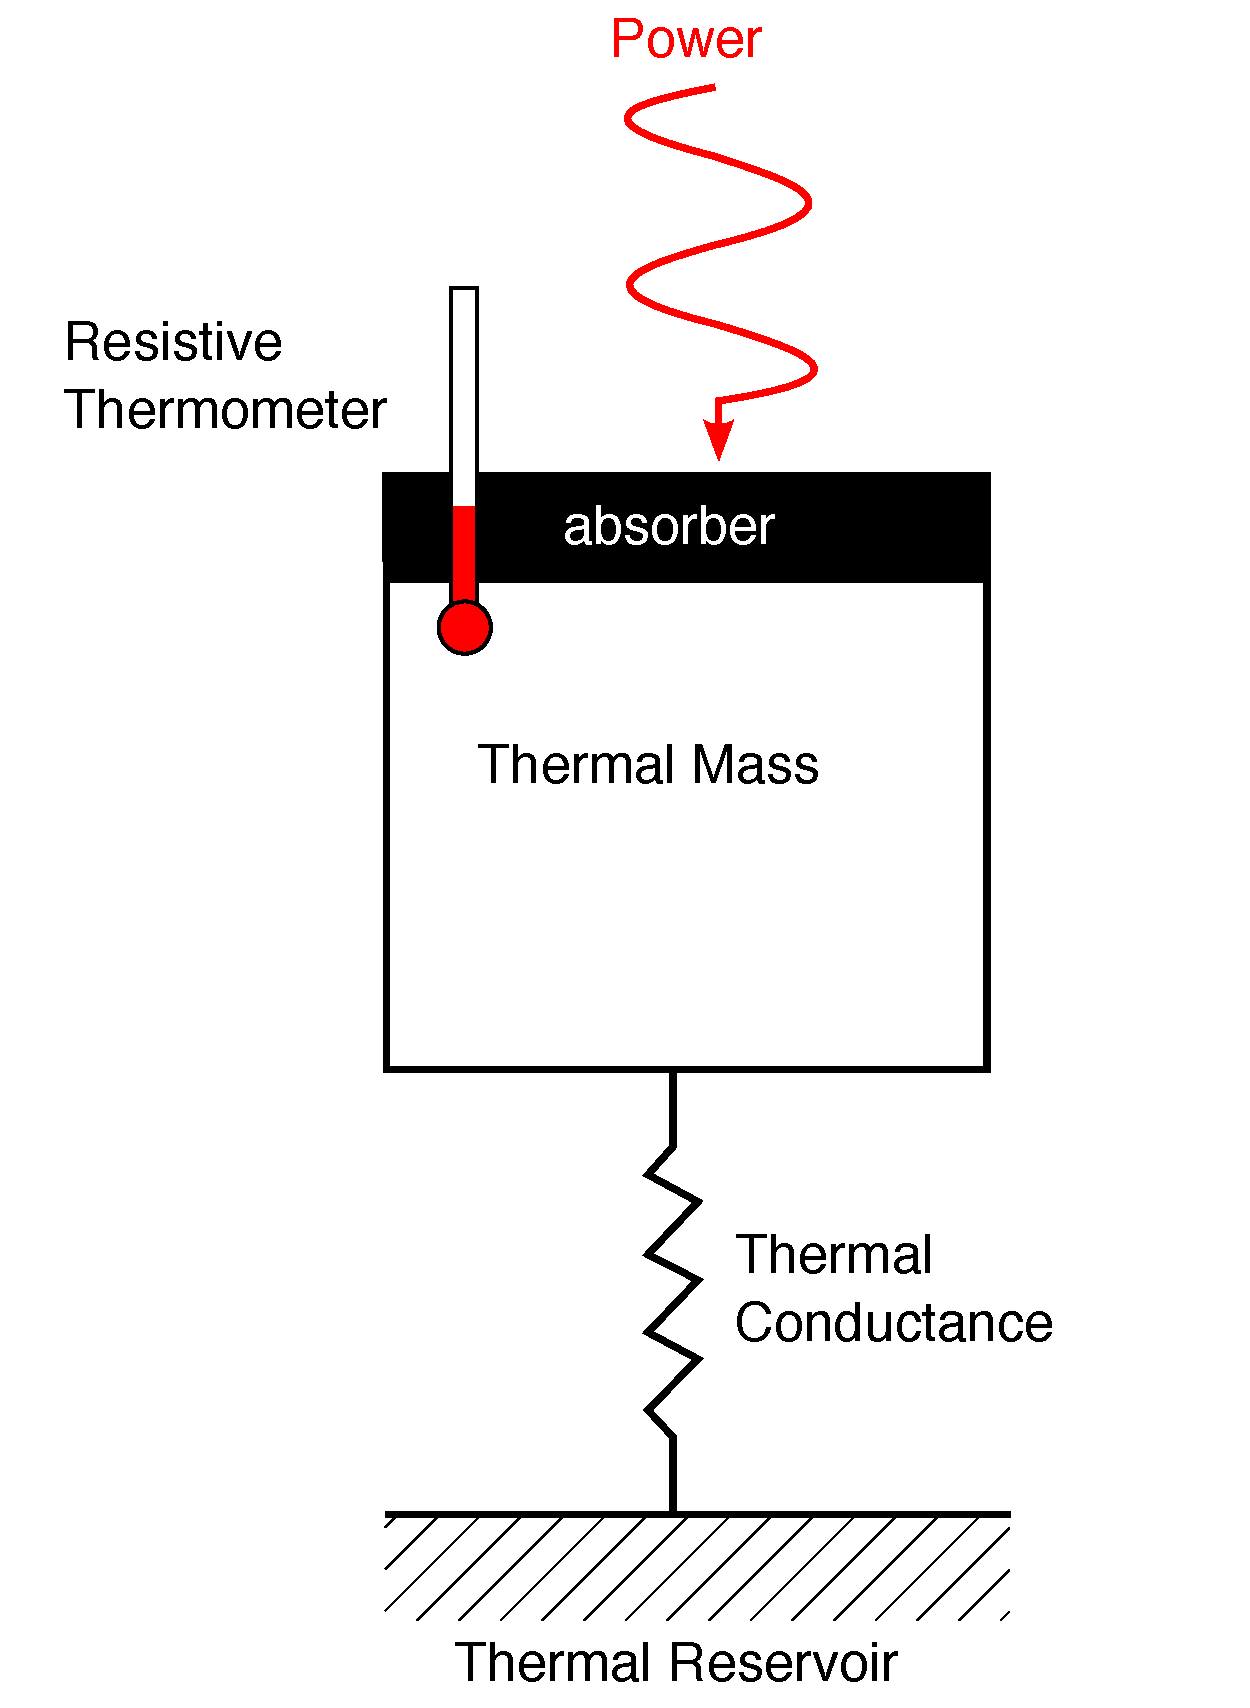
\includegraphics[width=0.8\linewidth]{figures/bolometer.pdf}
    \caption[Conceptual operation of a Bolometer]{Conceptual operation of a Bolometer \citep{bolometerSchematic}}
    \label{bolometer}
\end{figure}

While thermal noise is an issue for CCDs, it is a much bigger problem with bolometers. In order to get accurate readings, the whole device needs to be kept very cold, down to a below $100\units{mK}$ in some cases, and the time response for the thermal energy to flow into the thermal reservoir needs to be carefully calibrated and well understood for any particular device. Any thermal noise can easily drown out any useful signal measurable.

\subsection{Sampling Theory}

Information theory was developed in 1948 by Claude Shannon \citep{shannon2001mathematical} in order to find the fundamental limits of signal processing. The theory describes how much information is needed to convey some message through a communications channel, but the mathematics apply to how information can be sampled from some measurable phenomenon.

The theory was expanded into the field of digital signal processing, where it was established that the sampling rate required to obtain all the information from a continuous time signal is twice the highest frequency in the signal. So for instance to capture the signal from a pure sine wave at $1\units{Hz}$, measurements would need to be taken at a frequency of $2\units{Hz}$.

\subsection{Herschel Space Observatory}

The Herschel space observatory was launched by the ESA on the 14th of May, 2009, observing in the far infrared and submillimetre range of the EM spectrum, using a Cassegrain design with a $3.5\units{m}$ primary mirror. Herschel has two direct detection instruments, i.e. they measure the intensity of the incident radiation, PACS and SPIRE, and a high-resolution spectrometer, HIFI. The PACS imaging photometer observes at $70\units{\mu m}$, $100\units{\mu m}$ and $160\units{\mu m}$ and the SPIRE imaging photometer observes at 3 bands, $250\units{\mu m}$, $350\units{\mu m}$ and $500\units{\mu m}$ \citep{pilbratt2010herschel}. Note that combining the data from both PACS and SPIRE allows us to fit six data points to the blackbody spectrum. PACS and SPIRE also have spectrometers, although spectrographic data is not used in this project so these will not be discussed further.

\subsubsection{Herschel SPIRE}

\begin{figure}[H]
    \centering
    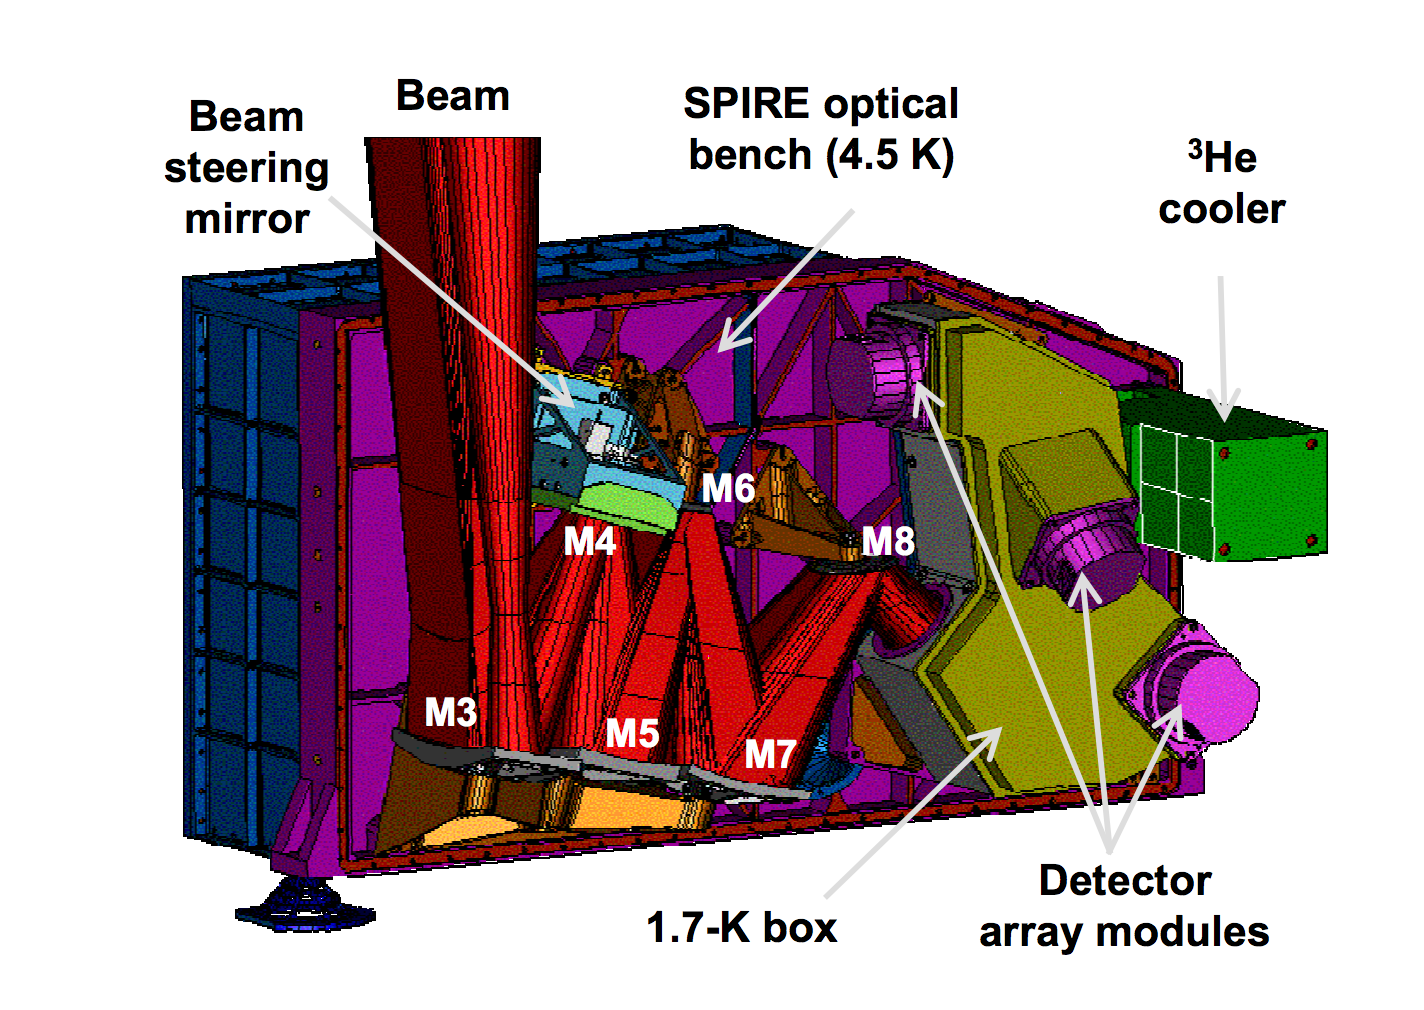
\includegraphics[width=0.8\linewidth]{figures/spire.png}
    \caption[SPIRE Photometer Layout]{SPIRE Photometer Layout \citep{griffin2010herschel}}
    \label{spire-schematic}
\end{figure}

The SPIRE instrument contains three arrays of bolometers cooled to $0.3\units{K}$. The photometer has a viewing field of 4'x8', observing simultaneously at $250\units{\mu m}$, $350\units{\mu m}$ and $500\units{\mu m}$ \citep{griffin2010herschel}. This corresponds to a diffraction limited resolution of 18'', 25'' and 36'' respectively.

Figure \ref{spire-schematic} shows the basic layout of the SPIRE optical system. SPIRE uses a series of mirrors to reflect the incoming beam onto the various instruments contained within, which are cooled by liquid $^3$He.

\begin{figure}[H]
    \centering
    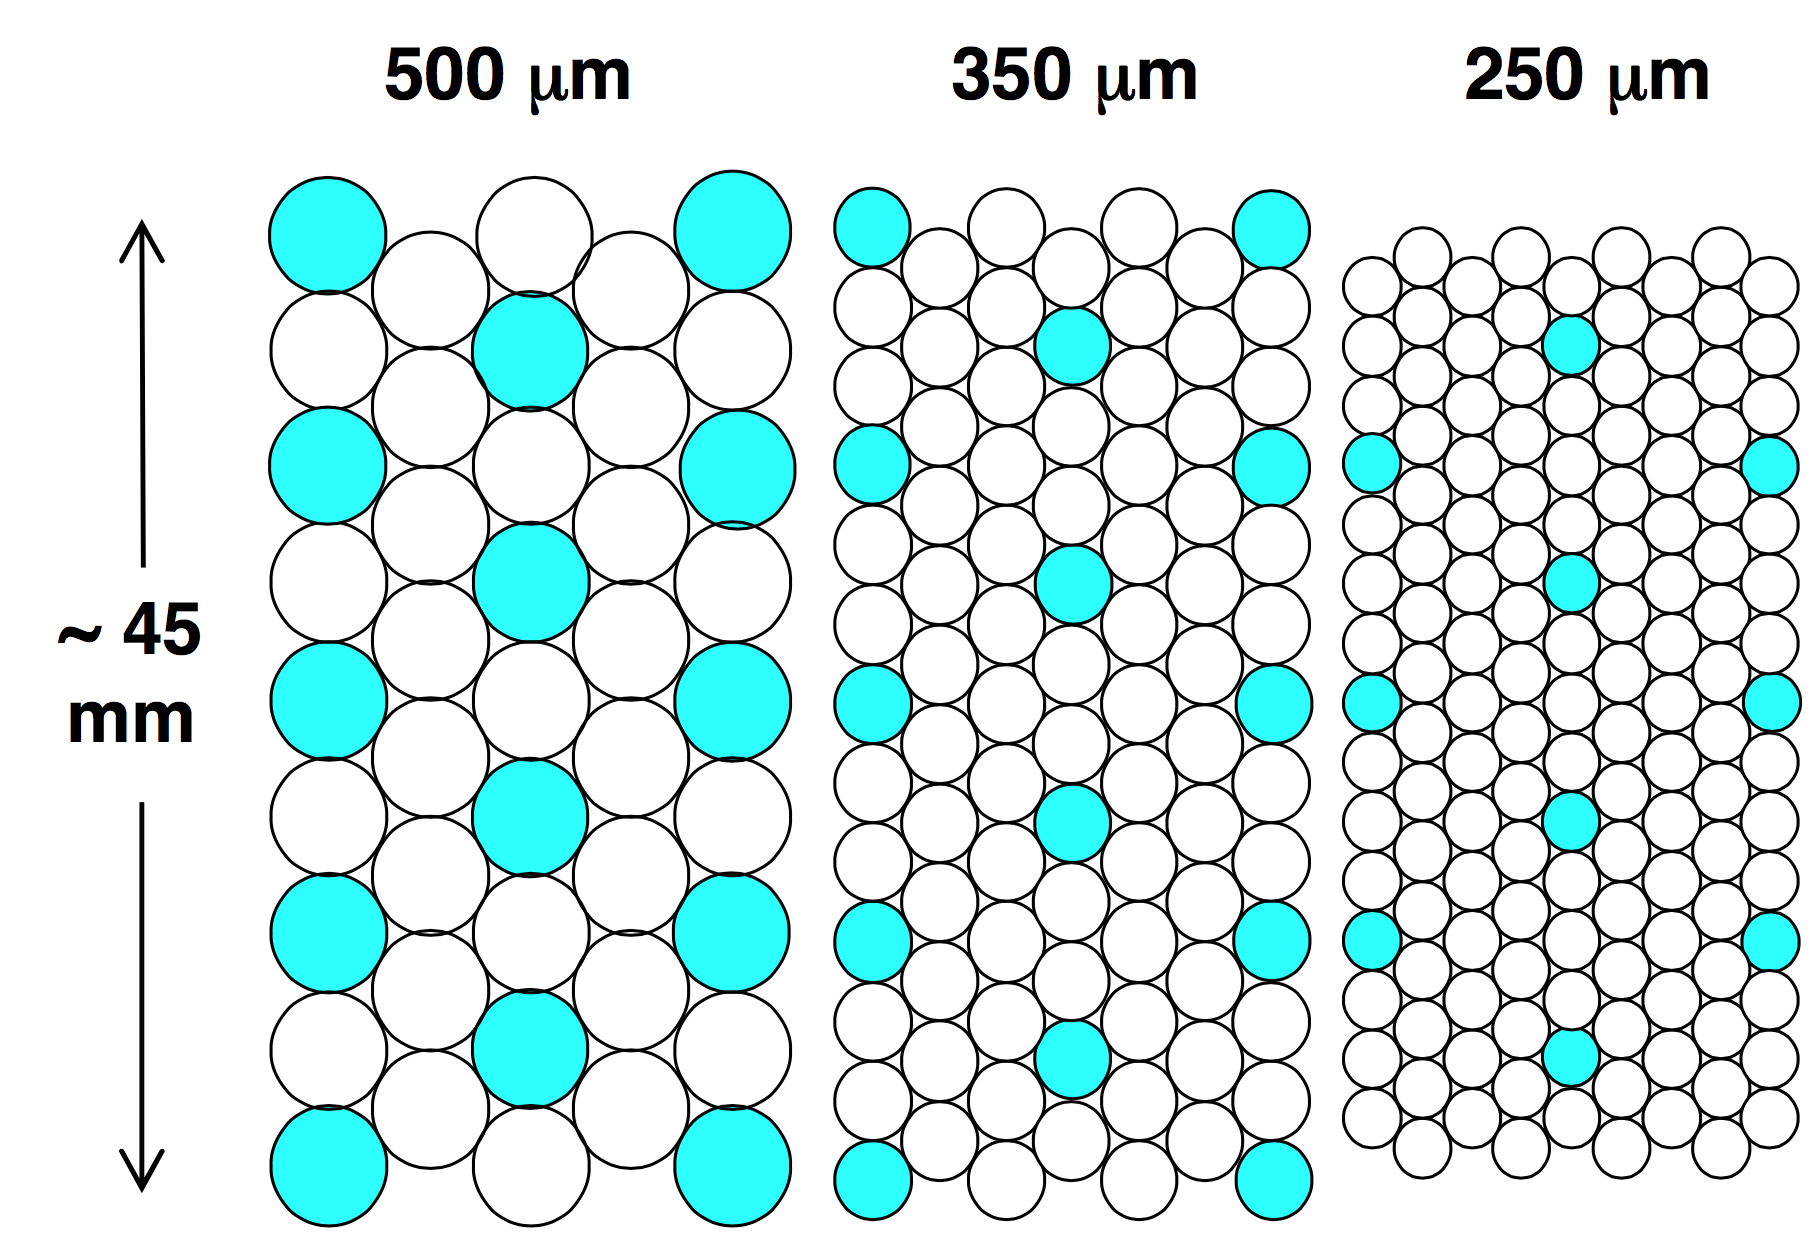
\includegraphics[width=0.8\linewidth]{figures/bolometer-layout.png}
    \caption[SPIRE Bolometer Array Layout]{SPIRE Bolometer Array Layout \citep{griffin2010herschel}}
    \label{spire-bolometer}
\end{figure}

There are three arrays of bolomerers for imaging. These arrays contain 43, 88 and 139 individual bolometers for the $500\units{\mu m}$, $350\units{\mu m}$ and $250\units{\mu m}$ band observations respectively, and are arranged as shown in Figure \ref{spire-bolometer}.

To achieve a larger field of view for observations, scans are taken across the sky, at a rate of $30''/s$ in the nominal mode, or $60''/s$ in fast mode \citep{handbook2014herschel}. The bolometer arrays are not fully filled, so the telescope scans are performed at $\pm42.4^\circ$ with respect to the Z-axis of the arrays, and the scan lines are separated by 348'' to provide overlap and good coverage. Cross scanning is performed at both the $\pm42.4^\circ$ angles providing full coverage and oversampling of the observation (Figure \ref{scan-angles}). The data for each bolometer is stored as a timeline and can later be processed into a map image.

\begin{figure}[H]
    \centering
    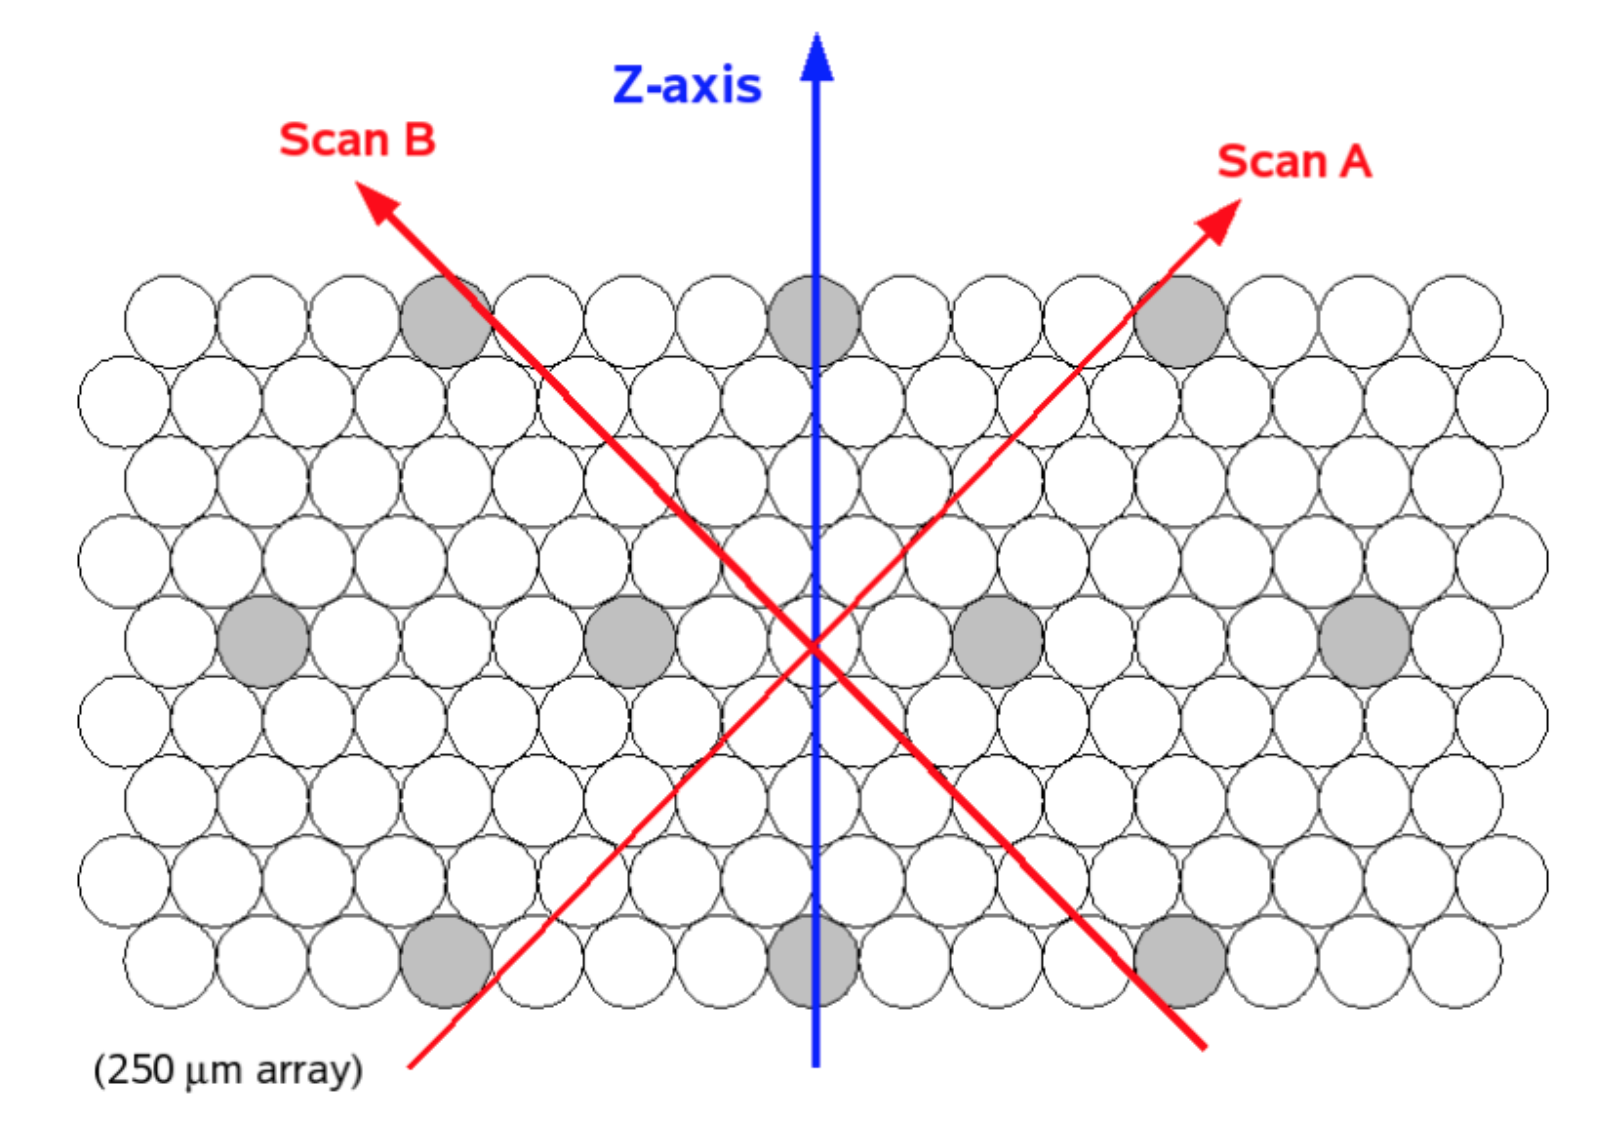
\includegraphics[width=0.8\linewidth]{figures/scan-angle.png}
    \caption[SPIRE map scan angles]{SPIRE map scan angles \citep{handbook2014herschel}}
    \label{scan-angles}
\end{figure}

The rate of sampling of this information into the timelines is greater than the limit required by Nyquist-Shannon sampling theory, and these signals are oversampled. It is this oversampling that allows for HiRes to achieve good results on the SPIRE observational data. With both PACS and SPIRE photometer data, a blackbody spectrum can be established for any observation, this is shown in Figure \ref{herschel-bb}.

\begin{figure}[H]
    \centering
    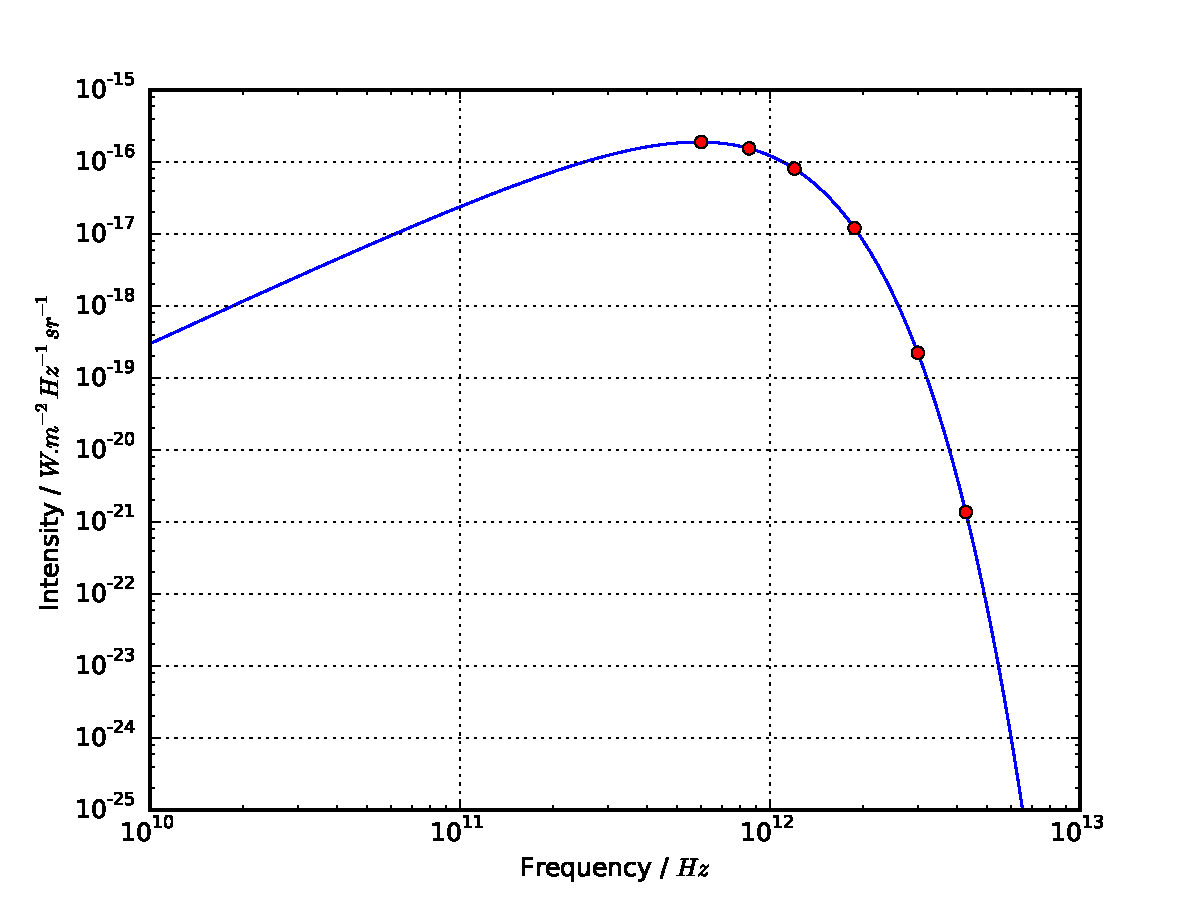
\includegraphics[width=\linewidth]{figures/bb10kHERSCHEL.pdf}
    \caption[Herschel observing frequencies for a 10K blackbody]{Herschel observing frequencies for a 10K blackbody combining both PACS and SPIRE photometers. The points show what would be the measured values for each photometer.}
    \label{herschel-bb}
\end{figure}

\subsection{Fourier Transformation}

A Fourier transform takes a source signal, and decomposes it into the various frequencies that make up that signal. In the case of a wave as a function of time, the Fourier transform will output the frequencies that make up that wave. In the case of an image the output will be the the spatial frequencies. Mathematically the Fourier of a transform is defined as in equation \ref{fft}, where $x$ is the independent variable in normal space, and $\mu$ is the transform variable in frequency space.

\begin{equation}
    f'(\mu) = \infint{ f(x) e^{-2\pi ix\mu}}{x}
    \label{fft}
\end{equation}

A Fourier transform can be reversed to give back the original function in normal space, using equation \ref{fftr}.

\begin{equation}
    f(x) = \infint{ f'  (\mu) e^{2\pi i\mu x}}{\mu}
    \label{fftr}
\end{equation}

\subsubsection{Discrete Fourier Transform}

While the Fourier transform as shown in equation \ref{fft} is useful when performing analytical analysis of some problem, it does not apply when some data set needs to be analyzed. In this case some other form is needed, and this suitable method to use is the discrete Fourier transform.

In a discrete Fourier transform, a set of samples of some function (i.e. the input data) is converted into a set of coefficients of sinusoids ordered by their respective frequencies. So for example, data sampled from a sine wave on the input function would generate a set of data with just a single value at the location of the frequency of the original sine wave.

The discrete Fourier transform is usually performed on a computer by what is known as a Fast Fourier Transform, which is usually an implementation of the Cooley-Tukey algorithm \citep{welch1967use}. Typically the fast Fourier transform routines return an image that has the same pixel dimensions as the source image, where the central pixel represents the lowest frequency component wave.

\subsection{Image Convolution}

Convolution is general method for filtering an image. A kernel is applied to each pixel of an image, and the output for each pixel is the sum of the piecewise multiplication of the kernel and the image. The kernel can be thought of as a matrix of pixel weights, and can be manipulated to produce many results, such as blurring, sharpening and edge detection on an image.

For example, an image may consist of a matrix of pixels with values:

\[
\begin{array}{|c|c|c|c|}
    \hline
0 & 0 & 0 & 0 \\
\hline
0 & 1 & 1 & 0 \\
\hline
0 & 0 & 0 & 0 \\
\hline
\end{array}
\]

And a convolution kernel of:

\[
\begin{array}{|c|c|c|}
    \hline
1 & -1 & 0 \\
\hline
1 & -1 & 0 \\
\hline
1 &  -1 & 0 \\
\hline
\end{array}
\]

By applying the kernel at each pixel location (and treating pixels beyond the edge as 0) would give the result:

\[
\begin{array}{|c|c|c|c|}
    \hline
0 & -1 & 0 & 1 \\
\hline
0 & -1 & 0 & 1 \\
\hline
0 & -1 & 0 & 1 \\
\hline
\end{array}
\]

\subsubsection{Fourier Convolution}

While performing convolution as described previously will produce a convolved image, it becomes a very time consuming operation as kernel size increases. There are also considerable difficulties with the implementation, especially with regard to convolving at the edges of an image.

There is however a solution to both of these problems. Convolution in real space corresponds directly to pointwise multiplication in the Fourier space, and deconvolution in real space to pointwise division in Fourier space \citep{katznelson2004introduction}. By performing any convolution or deconvolution in Fourier space, the time required to perform the convolution is taken almost entirely by the time performing the discrete Fourier transform. Modern data analysis libraries can perform the FFT operation incredibly fast, so when doing image convolutions with large kernels, such as a telescope beam image, Fourier convolution is usually the best choice of implementation method.

\subsection{HiRES Technique}

Originally used for data processing for the IRAS telescope launched in 1983 \citep{neugebauer1984infrared}, HiRes is a technique using the maximum correlation method to increase the fidelity of images above the nominal resolution \citep{aumann1990maximum}.

The diffraction limited resolution of the telescope can be overcome to some extent by reversing the process that limits the resolution. Essentially the image resolution is determined by a process which is essentially blurring the true sky image with the diffraction pattern produced by the telescope construction (the telescope beam). If we have a very accurate representation of this telescope beam, we can reverse this process by performing a Fourier deconvolution of the sampled image and the telescope beam \citep{lucy1974iterative}.

As HiRes is an MCM algorithm it can be applied before the image has been reconstructed from the timelines however, and operates on the data scans directly using a model of the detector response. By iterating the process it is possible to achieve significantly higher fidelity, although it is not yet clear where the limits of this technique lie with regards to SPIRE observations, nor under what conditions this method is suitable to use.
